\documentclass[conference]{IEEEtran}
\IEEEoverridecommandlockouts
% The preceding line is only needed to identify funding in the first footnote. If that is unneeded, please comment it out.
\usepackage{cite}
\usepackage{amsmath,amssymb,amsfonts}
\usepackage{algorithmic}
\usepackage{graphicx}
\usepackage{textcomp}
\usepackage{xcolor}

\usepackage{setspace}
\usepackage[T1]{fontenc}
\usepackage{url}
\usepackage{hyperref}
\usepackage{enumitem}
\usepackage{mathtools}
\def\BibTeX{{\rm B\kern-.05em{\sc i\kern-.025em b}\kern-.08em
		T\kern-.1667em\lower.7ex\hbox{E}\kern-.125emX}
}
\newcounter{boxlblcounter}  
\newcommand{\makeboxlabel}[1]{{#1.}\hfill}% \hfill fills the label box
\newenvironment{boxlabel}
{\begin{list}
		{\arabic{boxlblcounter}}
		{\usecounter{boxlblcounter}
%			\setlength{\labelwidth}{3em}
%			\setlength{\labelsep}{0em}
			\setlength{\itemsep}{2pt}
			\setlength{\leftmargin}{1cm}
%%			\setlength{\rightmargin}{2cm}
%			\setlength{\itemindent}{0em} 
			\let\makelabel=\makeboxlabel
		}
	}
{\end{list}}
\usepackage{caption}

\usepackage{bookmark}
\usepackage{array}
\usepackage{listings}
\usepackage{float}
\usepackage{pifont}% http://ctan.org/pkg/pifont
\newcommand{\xmark}{\ding{55}}%

\begin{document}
	
	%%
	%% Modified title page for UA
	\begin{titlepage}
	\begin{figure}[t]
		\begin{minipage}{\textwidth}
			\centering
			
\includegraphics[scale=0.35]{Images/UA/OfficLogo-Engineering.png}
		\end{minipage}
	\end{figure}

	\quad\\
	\vspace{0.5in}
	\centering
	\begin{spacing}{2.0}
		{ \textbf{\LARGE AVoIP: Ad-Hoc Voice over Internet Protocol for Small Single-board Computers}}
	\end{spacing}
	
	\vspace{1.5in}
	\textbf{\Large Term Project Proposal}
	\vspace{3.0in}

	\begin{minipage}{0.49\textwidth}
		\begin{flushleft}
			\textit{{Students:}} \\
			{\textbf{Trupeshkumar R. Patel}}\\
			\textsl{trpatel2@crimson.ua.edu}\\
			{\textbf{David Coleman}}\\
			\textsl{dmcoleman1@crimson.ua.edu}\\
			{\textbf{Xiaoming Guo}}\\
			\textsl{xguo29@crimson.ua.edu}
		\end{flushleft}
	\end{minipage}
	\begin{minipage}{0.5\textwidth}
		\begin{flushright}
			\textit{{Supervisor:}} \\
			{\textbf{Dr. Xiaoyan Hong}}\\
			\textsl{hxy@cs.ua.edu}
		\end{flushright}
	\end{minipage}

	\begin{figure}[b]
		\begin{minipage}{0.55\textwidth}
			\begin{flushleft}
				\textbf{\large Department of Computer Science}
			\end{flushleft}
		\end{minipage}
		\hfill
		\begin{minipage}{0.35\textwidth}
			\begin{flushright}
				\textsc{\textbf{\today}}
			\end{flushright}
		\end{minipage}
	\end{figure}

\end{titlepage}
	
	%%
	%% The "title" command has an optional parameter,
	%% allowing the author to define a "short title" to be used in page headers.
	\title{AVoIP: Ad-Hoc Voice over Internet Protocol for Small Single-board Computers}
	\IEEEspecialpapernotice{(Checkpoint Report)}
	%%
	%% The "author" command and its associated commands are used to define
	%% the authors and their affiliations.
	%% Of note is the shared affiliation of the first two authors, and the
	%% "authornote" and "authornotemark" commands
	%% used to denote shared contribution to the research.
	%\author{
%	\IEEEauthorblockN{Trupesh R. Patel}
%	\IEEEauthorblockA{
%		Department of Computer Science\\
%		College of Engineering\\
%		\textit{University of Alabama}\\
%		Tuscaloosa, AL 35487\\
%		trpatel2@crimson.ua.edu\\
%%		\orcid{0000-0003-4321-6699}
%	}
%
%	\and
%	
%	\IEEEauthorblockN{Author 1}
%	\IEEEauthorblockA{
%		Department
%		\textit{University of Alabama}\\
%		Tuscaloosa, AL 35487\\
%		email@email.com
%%		\orcid{0000-0003-4321-6699}
%	}
%
%	\and
%	
%	\IEEEauthorblockN{Author 2}
%	\IEEEauthorblockA{
%		Department
%		\textit{University of Alabama}\\
%		Tuscaloosa, AL 35487\\
%		email@email.com
%		%		\orcid{0000-0003-4321-6699}
%	}
%}



\author{
	\IEEEauthorblockN{
		Trupesh R. Patel\IEEEauthorrefmark{1}, 
		David Coleman\IEEEauthorrefmark{1}, 
		Xiaoming Guo\IEEEauthorrefmark{1}
	} 
	\IEEEauthorblockA{
		\IEEEauthorrefmark{1}Department of Computer Science\\
					College of Engineering\\
					\textit{University of Alabama}\\
					Tuscaloosa, AL 35487\\
					$\left\{trpatel2,\ dmcoleman1,\ xguo29\right\}$@crimson.ua.edu
	} 
}


	
	%%
	%% This command processes the author and affiliation and title
	%% information and builds the first part of the formatted document.
	\maketitle
	\thispagestyle{plain}
	\pagestyle{plain}
	
	%%
	%% The Objective is a short summary of the work to be presented in the
	%% article.
%	{
	\bfseries\textit{Objective}---
	Asterisk PBX is a software implementation of Private Branch Exchange (PBX), a system used to handle telecommunication services, allowing VoIP (Voice over Internet Protocol) services on computers, including less powerful devices such as Raspberry Pi. However, using smaller single-board devices come with the limitation of computing power and storage capacity. As a result of these limitations are dropping packets, cutting off the callers while handling a more significant number of calls simultaneously. In this project, the authors propose running a distributed Raspberry Pi model over an ad-hoc network with an Asterisk PBX system to determine how well VoIP services work within a distributed single-board system. Then this network configuration will be tested for the maximum number of calls, packets delays, network jitters, end-to-end network latency, and bandwidth as work shared between multiple Raspberry Pi.
%	Asterisk PBX is a software implmentation of Private Branch Exchange, a system used to handle telecommunication services. This allows for the usage of Voice over IP services on computers, including less powerful devices running on Raspberry Pis.	A limitation of using weaker devices to run Asterisk PBX is that computers with little memory or weak CPUs can quickly be overwhelmed when having to deal with a large number of callers at once, cutting off callers and dropping many packets.	In this proposal, the work required to run Asterisk PBX will be distributed over an ad hoc network of Raspberry Pis, to determine how well VoIP services work within a distributed single board system.	This configuration will be tested for maximum callers that the network can handle, delays with high number of callers, and increaed latency as work is shared between the Raspberry Pis.
}
	
	
	%%
	%% Keywords. The author(s) should pick words that accurately describe
	%% the work being presented. Separate the keywords with commas.
%	\begin{IEEEkeywords}
%		abc
%	\end{IEEEkeywords}
	
	%%
	%% The introdution section
\section{Introduction \& Background}	
\label{sec:introduction-background}
Voices can have multiple functions among the information flowing at the edge of the IoT network. They can carry valuable content, reflect the conditions of an environment, and can be used to command other entities through acoustic actuators and phone calls. However, implementing voice systems at the edge of such networks typically faces challenges, namely that edge devices are always constrained by computing power, bandwidth contention, and energy consumption. Therefore, it is not feasible to implement a complete TCP/IP stack on each node and give all nodes the ability to connect to remote entities outside the local network.

IP-PBX (IP-based Private Branch Exchange) provides a comprehensive solution to address the aforementioned issues. As the analog equivalent of IP PBX, the design of the traditional PBX system is to serve a private organization, in which both the geographic area and the communication connection are limited to a specific scope. Connections between internal phones are without cost, while only central office lines provide connections to the public switched telephone network (PSTN). This scheme meets our expectations for edge IoT communication -- internal communication does not occupy egress bandwidth, and some switcher servers still reserve the communication egress to the outside. Leveraging VoIP technology, IP-PBX has ported the PBX scheme to the Internet, replacing telephone lines with packet-switching networks. The IP-based paradigm offers better scalability and lowers the cost same as the Internet brings to other domains. 

Several mature implementations of the IP-PBX paradigm are available, including 3CX~\cite{3cx_2022} and Asterisk PBX~\cite{sangoma-technologies}. Asterisk is an open-source software package that can run all PBX functions, along with some other functions, usually on a Linux operating system platform. Voicemail services, conference calling, interactive voice response, and call queuing are provided by Asterisk, along with the essential telephony services. It also provides multi-party calling and displaying of caller ID (display calling number). To interact with digital telephone equipment and analog telephone equipment, Asterisk needs the support of PCI hardware, the most famous of which is provided by the Digium platform. 

From the architecture perspective, Asterisk serves as a middleware function, connecting the underlying telephony technology and the upper-level telephony applications. Both PBX and IVR (Interactive Voice Response) functionalities are integrated within Asterisk. Using compatible PCI hardware, Asterisk supports traditional telephone lines, including TDM (Time Division Multiplexing), TI/El PRI/PRA\&RBS (Robbed Bit Signal) mode, analog telephone line/analog telephone (POTS), ISDN (Integrated Services Digital Network) and BRI (Basic Rate) and PRI (Primary Rate). Also, due to the PCI hardware support feature, Raspberry Pi can be used to implement the Asterisk instance. 

By using small single-board computers such as Raspberry Pi, any types of businesses can deploy the cost affordable IP based PBX system. Raspberry Pi is small and light weight device, and runs on low power consumption. Having it for single tasks like allowing for VoIP by running Asterisk PBX is a very easy and economical. However, because this device is smaller and lighter, it can only handle a limited number of tasks. This paper will analyze the boundaries of the Raspberry Pi by packets delays, network jitters, end-to-end network latency, and bandwidth of calls made at varying distances from the Pi to determine how effectively IP-PBX services can be run on such devices.
	
This paper is organized into specific sections. \hyperref[sec:setup]{Section \ref{sec:setup}} lists the required hardware and software involved with the experiments performed here.  \hyperref[sec:obstacles]{Section \ref{sec:obstacles}} explains the obstacles faced when setting up for the tests in this experiment. \hyperref[sec:analysis-methods]{Section \ref{sec:analysis-methods}} explains the protocols that Asterisk PBX is using to connect devices and forward calls, how the calls are impacted by different network issues, and what topology IP-PBX services utilize to connect devices. \hyperref[sec:experiments]{Section \ref{sec:experiments}} shows detailed description for each experiment performed. \hyperref[sec:future-work]{Section \ref{sec:future-work}} goes over different ways the material of this paper can be expanded upon in the future. Finally, \hyperref[sec:conclusion]{Section \ref{sec:conclusion}} concludes the paper, giving an overview of the results seen thus far.

\section{Experiment}	
\label{sec:sip}


\subsection{Basic SIP Analysis}

The Session Initiation Protocol (SIP) is an application layer control protocol for establishing, changing and terminating multimedia sessions, where the sessions can be IP telephony, multimedia sessions or multimedia conferences. SIP is the core protocol of many IP-based PBX applications, including Asterisk.

To demonstrate the main components of the SIP communication, a simplified scenario is implemented, as shown in Figure \ref{fig:topo}. Two softphone applications are running on the same computer, and an IP-based PBX application (Asterisk), running on a Raspberry Pi 4, is serving as the PBX server.

\begin{figure}[htbp]
\centerline{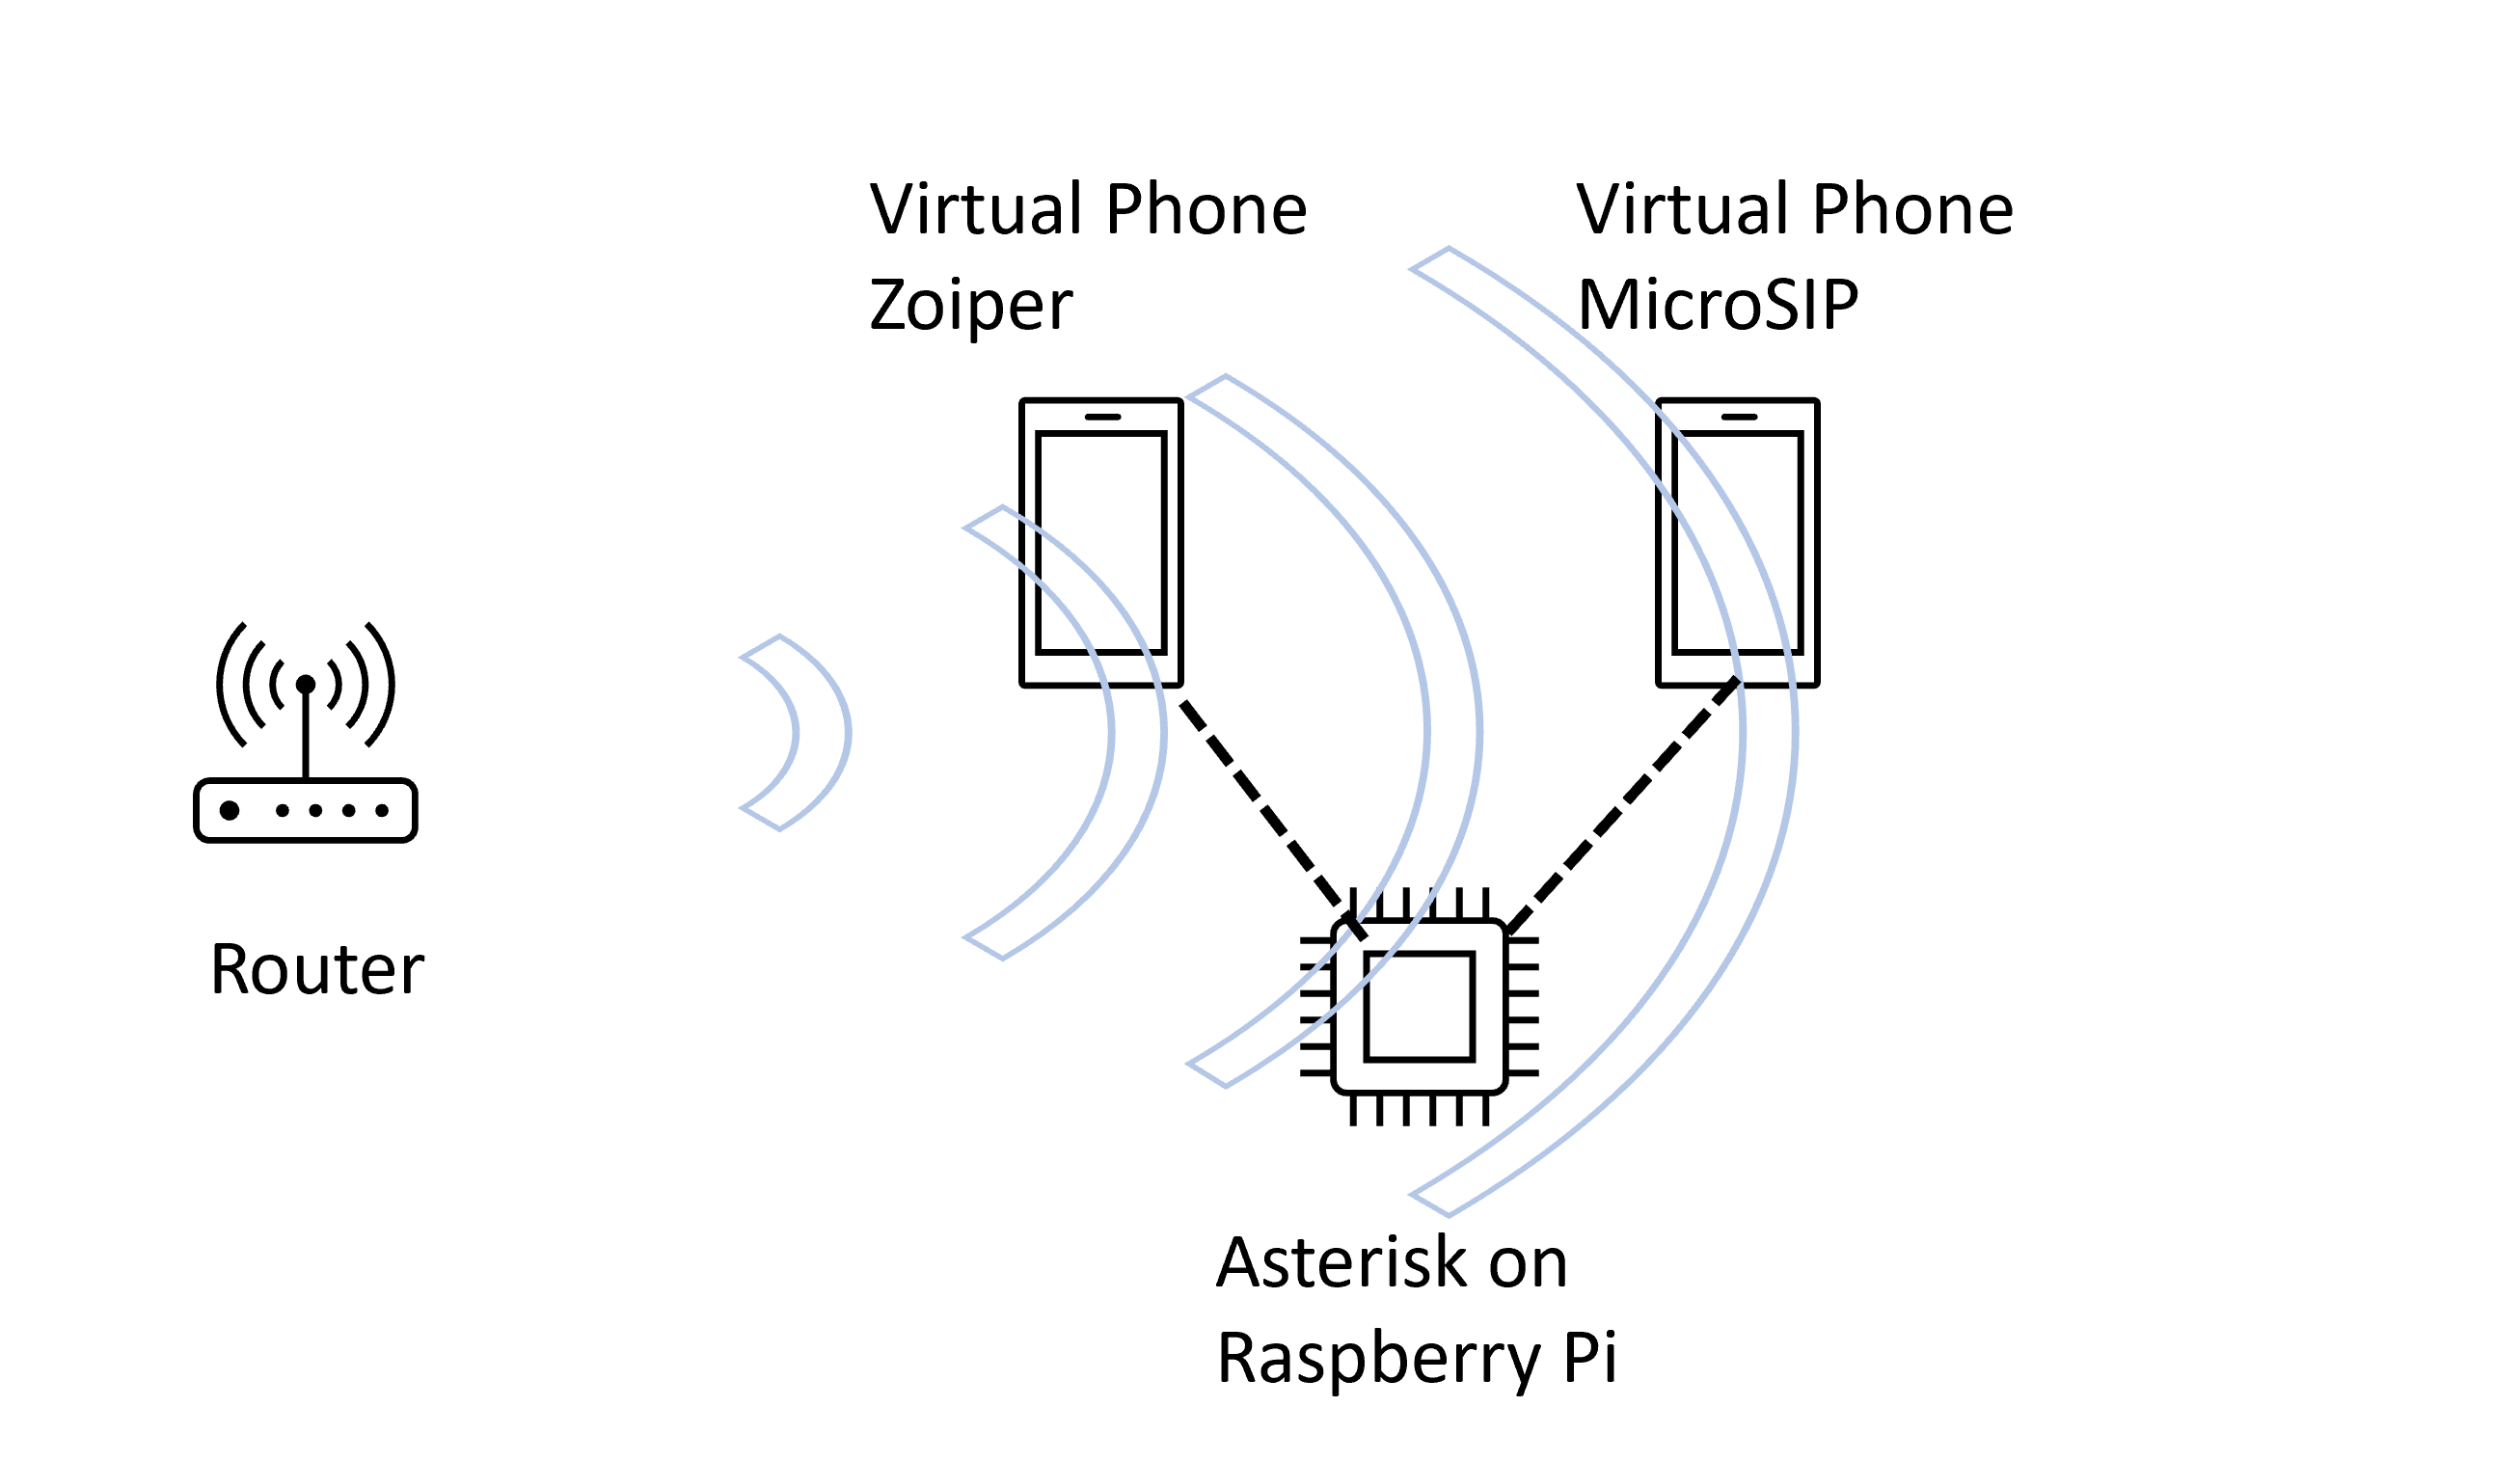
\includegraphics[width=8cm]{Images/experiment/exp1.png}}
\caption{Simplified Scenario}
\label{fig:topo}
\end{figure}

The SIP process starts with registration. All SIP terminals as User Agents should register with the registration server to inform their location, session capability, and other information.

Usually, when the SIP terminal (User Agent) is powered on or configured to perform a registration operation, a registration request message (REGISTER) is sent to the registration server, carrying all the information that needs to be registered. After receiving the registration request message, the registration server sends a response message to the terminal to inform it that the request message has been received. If the registration is successful, it will send a "200 OK" message to the terminal. However, the most common response is a "401 Unauthorized" message because authorization is required in most of the implantations for security purposes. As shown in Figure 2.


The SIP protocol adopts the Client-Server pattern, in which the calls are established between User Agents through the proxy server.


\begin{figure}[htbp]
  \centering
  \begin{minipage}[b]{0.3\textwidth}
    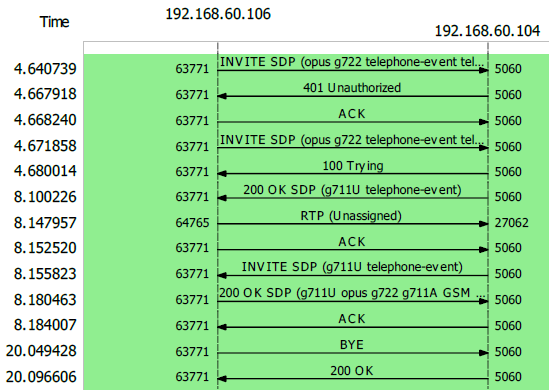
\includegraphics[width=\textwidth]{Images/experiment/a1.png}
    \caption{Zoiper to Asterisk}
  \end{minipage}
  \hfill
  \begin{minipage}[b]{0.3\textwidth}
    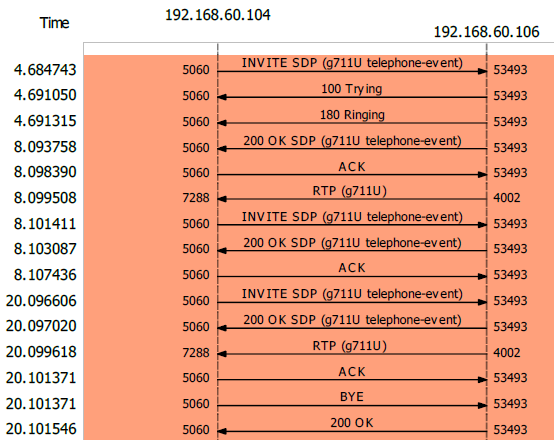
\includegraphics[width=\textwidth]{Images/experiment/a2.png}
    \caption{Zoiper to MicroSIP}
  \end{minipage}
\end{figure}



	%%
	%% The timel;ine and milestone section
%	\section{Timeline \&Milestones}	\label{sec:timeline-milestone}
	Text here.	
	
	%%
	%% The analysis  section
%	\section{Analysis}	\label{sec:analysis}
	Text here.
	
	%%
	%% The synthesis  section
%	\section{Synthesis} \label{sec:synthesis}
	Text here.
	
	%%
	%% The state of the art section
%	\section{State of the Art}
	Text here.
	
	%%
	%% The future directions  section
%	\section{Future Work} \label{sec:future-work}
    While this may act as a basic foundation for proving the efficacy of the Raspberry Pi as a cheap means to implement IP-PBX software, there are several means of expanding upon this work.
    \subsection{Further Testing}
        More experiments can be performed to determine the limitations that Raspberry Pis can prove to have when running IP-PBX software. A major test would be stressing the Pi by seeing how many calls it can handle in situations where bandwidth is plentiful, with the CPU and RAM of the Pi being the major bottlenecks at that point. This same test could be performed using different models of the Pi to see how the difference in CPU and RAM can affect VoIP calls. Analyzing this data could provide a way to determine the best board to purchase based on how many calls are needed to be handled.
        
        A limitation of data for outside network calls restricts current analysis. Future studies could attempt to have separate Raspberry Pis running PBX software on different networks, while allowing VoIP calls to be made between them. Data could then be collected based on test calls between these IP-PBX instances. This would prove useful in analyzing the effectiveness of the Pi in making outside network calls.
    \subsection{Horizontal Scaling}
        A powerful characteristic of cheap computers such as a Raspberry Pi is their suitability for horizontal scaling. If an institution grows large enough that one Pi cannot handle the all of the institution's VoIP calls, there are two methods of scaling up the memory and processing power available for IP-PBX services. The first is to scale the system vertically; replace the Pi with a single, more powerful computer with more memory, and either sell the Pi or reuse it for some other purpose. The second is to scale the system horizontally; connect more Raspberry Pis with the original and have them share the workload of the VoIP calls. As Raspberry Pis are inexpensive, this allows for a cheaper alternative to buying a more powerful computer. Further works can delve into whether this is a possible technique to implement with IP-PBX software, and whether or not horizontal scaling provides many benefits for IP-PBX services.
	
	%%
	%% The Conclusion section
%	\section{Conclusion} \label{sec:conclusion}
    A single Raspberry Pi with 4GB of RAM is quite capable of running IP-PBX software without any noticeable issues. However, configuring the software to allow for VoIP calls can be quite complicated, and requires a great deal of outside instruction to fully understand. As well, a vital component of using the Raspberry Pi for these purposes is considering the network involved. If the Pi or VoIP devices are in areas with weak signal strength, jitter can grow rapidly, packet loss can begin to noticeably occur, connections can be dropped abruptly, and delays can become much more noticeable. If these effects occur, either due to weak signal strength or due to other possible issues, call quality can suffer dramatically. Consideration is required to install a usable and useful IP-PBX system for VoIP calls.
	%%
	%% The acknowledgments section
%	\section*{Acknowledgment}
	Text here.
	
	%%
	%% The next two lines define the bibliography style to be used, and
	%% the bibliography file.
%	\bibliographystyle{IEEEtran}
%	\bibliography{ref}
	
	%%
	%% If your work has an appendix, this is the place to put it.
%	\appendix
	
\end{document}